\section{Cursograma Pagos a Proveedores}
\begin{center}
 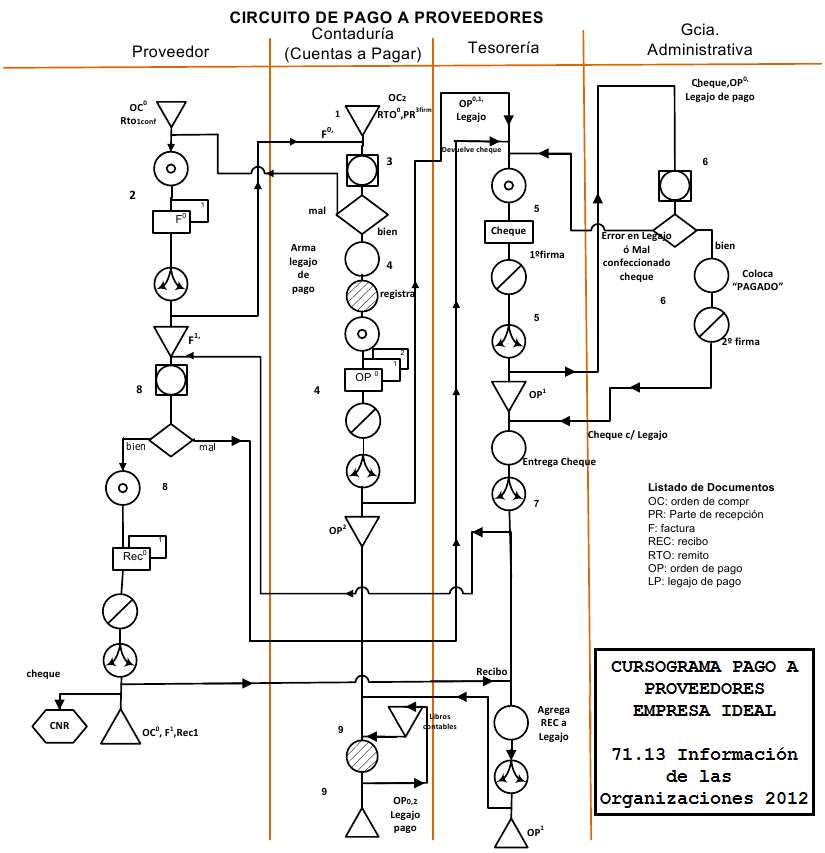
\includegraphics[scale=0.7,keepaspectratio=true]{./Circuitos-Teoricos/Pago-a-Proveedores/Images/cursograma-pago-a-proveedores.png}
 % cursograma-pago-a-proveedores.png: 587x630 pixel, 96dpi, 15.53x16.67 cm, bb=0 0 440 472
\end{center}

\section{Procedimiento de Pagos a Proveedores}
\begin{center}
 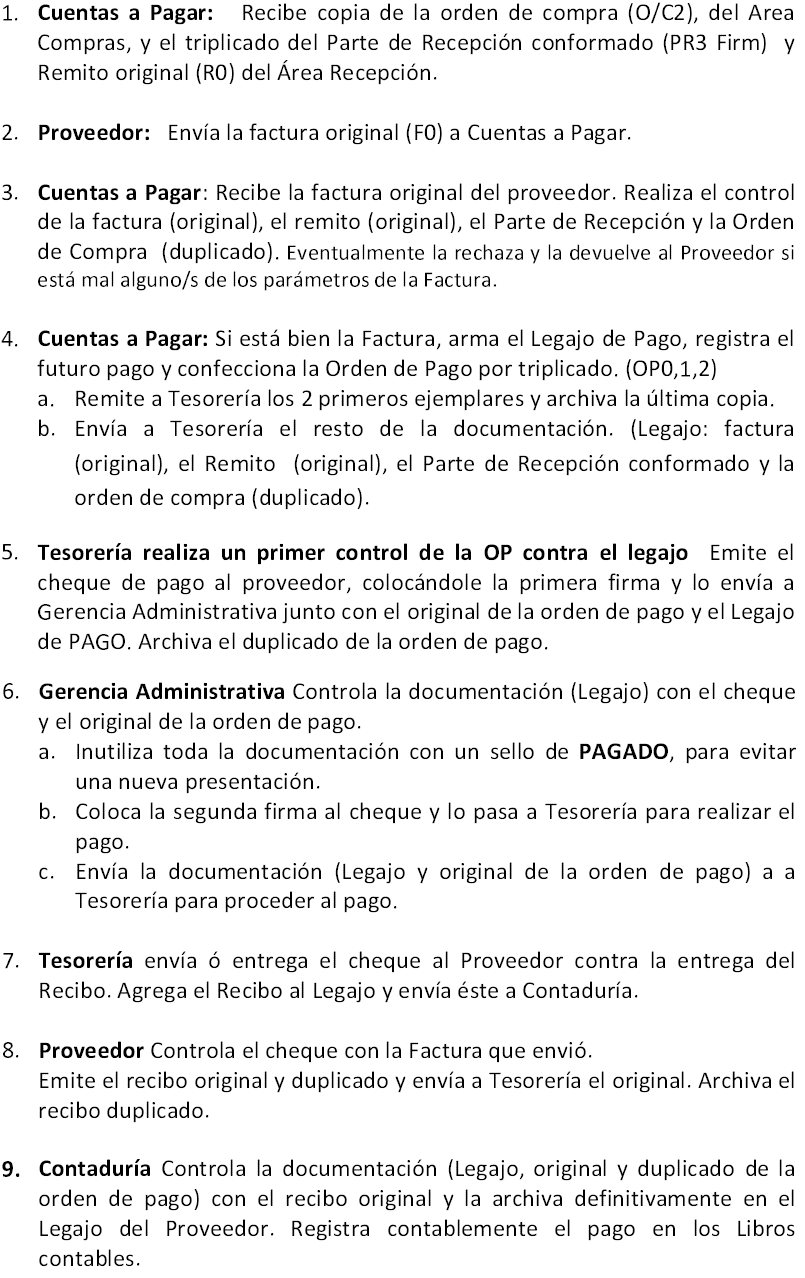
\includegraphics[scale=0.7,keepaspectratio=true]{./Circuitos-Teoricos/Pago-a-Proveedores/Images/procedimiento-pago-a-proveedores.png}
 % procedimiento-pago-a-proveedores-1.png: 805x927 pixel, 96dpi, 21.30x24.52 cm, bb=0 0 604 695
\end{center}

\section{Cursograma de Pagos (con numeración para el manual)}
\subsection{Manual del Cursograma de Pagos}

\begin{center}\textbf{Sectores intervinientes}\end{center}
\begin{itemize}
  \item Proveedor
  \item Contaduría (Cuentas a pagar)
  \item Tesorería
  \item Gcia. Administrativa
\end{itemize}

\begin{center}
  \textbf{Emisión de Documentos}
  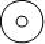
\includegraphics{./Images/Simbolos/simbolo-Emision-de-Documentos.png}
\end{center}
\begin{enumerate}
  \item Proveedor emite factura, original y copia
  \item Proveedor emite recibo del pago, en original y duplicado.
  \item Cuentas a pagar, de acuerdo a la factura recibida, confecciona la Orden de Pago por triplicado.
  \item Tesorería emite cheque de pago a proveedor.
\end{enumerate}

\begin{center}
  \textbf{Documentos}
  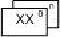
\includegraphics{./Images/Simbolos/simbolo-Documentos.png}
\end{center}
\begin{enumerate}
  \item Factura (F).
  \item Recibo (REC)
  \item Orden de pago (OP).
  \item Cheque
\end{enumerate}

\begin{center}
  \textbf{Distribución}
  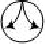
\includegraphics{./Images/Simbolos/simbolo-Distribucion.png}
\end{center}
\begin{enumerate}
  \item Proveedor distribuye factura original a cuentas a pagar, y conserva el duplicado.
  \item Proveedor distribuye recibo original a Tesorería, conserva el duplicado.
  \item Cuentas a Pagar distribuye las órdenes de pago. Original y duplicado a Tesorería, conserva el triplicado.
  \item Tesorería distribuye cheque, orden de pago original y legajo de pago a Gcia. Administrativa.
  \item Tesorería distribuye cheque a proveedor, previamente lo registra.
  \item Tesorería distribuye Recibo y Legajo a Contaduría.
\end{enumerate}

\begin{center}
  \textbf{Firma}
  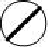
\includegraphics{./Images/Simbolos/simbolo-Firma.png}
\end{center}
\begin{enumerate}
  \item Proveedor firma recibo.
  \item Cuentas a Pagar firma las órdenes de pago.
  \item Tesorería pone la primera firma en el cheque.
  \item Gcia. administrativa pone la segunda firma en el cheque.
\end{enumerate}

\begin{center}
  \textbf{Almacenamiento Transitorio}
  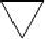
\includegraphics{./Images/Simbolos/simbolo-Almacenamiento-Transitorio.png}
\end{center}
\begin{enumerate}
  \item Cuentas a Pagar almacena OC2, RTO0 y PR3firm .
  \item Cuentas a Pagar almacena OP2.
  \item Cuentas a Pagar almacena libros contables.
  \item Tesorería almacena OP1.
\end{enumerate}

\begin{center}
  \textbf{Control y verificación}
  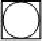
\includegraphics{./Images/Simbolos/simbolo-Control-y-Verificacion.png}
\end{center}
\begin{enumerate}
  \item Proveedor controla el cheque con la factura que envió, para verificar el cumplimiento del pago de la misma, verificando el monto y el plazo de pago.
  \item Cuentas a Pagar realiza control de factura, remito, parte de recepción y la orden de compra, verificando que la factura haya sido correctamente confeccionada, y que tanto ésta última como el remito y el parte de recepción referencien a la orden de compra en cuestión. 
  \item Gcia. administrativa controla el legajo con el cheque y el original de la orden de pago, verificando que el cheque haya sido correctamente confeccionado, para el proveedor en cuestión y con el monto correcto.
\end{enumerate}

\begin{center}
  \textbf{Decisión}
  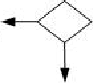
\includegraphics{./Images/Simbolos/simbolo-Decision.png}
\end{center}
\begin{enumerate}
  \item Proveedor si el cheque pasa el control y verificaci\'on, entonces se emite el recibo; caso contrario devuelve el cheque a Tesorería.
  \item Cuentas a Pagar si la factura pasa el control y verificaci\'on, entonces arma el legajo de pago; caso contrario rechaza la factura y la devuelve al proveedor.
  \item Gcia. administrativa si legajo pasa el control y verificaci\'on, entonces coloca PAGADO y firma el cheque; caso contrario devuelve la documentación a Tesorería.
\end{enumerate}

\begin{center}
  \textbf{Almacenamiento definitivo}
  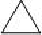
\includegraphics{./Images/Simbolos/simbolo-Almacenamiento-Definitivo.png}
\end{center}
\begin{enumerate}
  \item Proveedor almacena definitivamente OC0, F1 y Rec1
  \item Cuentas a Pagar almacena definitivamente OP0, 2, y Legajo de pago.
  \item Tesorería almacena definitivamente OP1
\end{enumerate}

\begin{center}
  \textbf{Operación}
  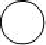
\includegraphics{./Images/Simbolos/simbolo-Operacion.png}
\end{center}
\begin{enumerate}
  \item Cuentas a Pagar arma legajo de pago.
  \item Tesorería entrega cheque.
  \item Tesorería agrega el recibo al legajo de pago.
  \item Gcia. administrativa coloca “Pagado” inutilizando toda la documentación, para evitar nueva presentación.
\end{enumerate}

\begin{center}
  \textbf{Registro}
  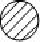
\includegraphics{./Images/Simbolos/simbolo-Registro.png}
\end{center}
\begin{enumerate}
  \item Cuentas a Pagar registra la compra en la cta. cte. proveedores.
  \item Cuentas a Pagar registra contablemente el pago en los libros contables. 
\end{enumerate}

\begin{center}
  \textbf{Circuito no relevado}
  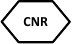
\includegraphics{./Images/Simbolos/simbolo-CNR.png}
  % simbolo-CNR.png: 73x44 pixel, 96dpi, 1.93x1.16 cm, bb=0 0 55 33
\end{center}
\begin{enumerate}
  \item Cobranzas (circuito del proveedor).
\end{enumerate}

\pagebreak
\section{Formularios de Pagos a Proveedores}
\subsection{Orden de Pago} 

\begin{center}
 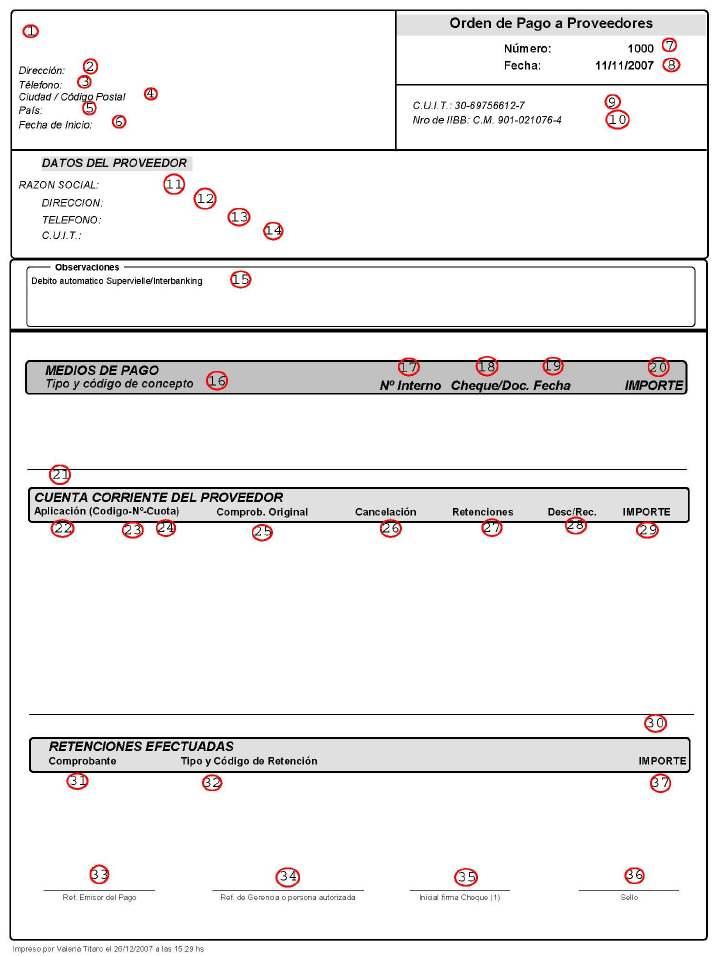
\includegraphics[scale=0.8,keepaspectratio=true]{./Circuitos-Teoricos/Pago-a-Proveedores/Images/orden-de-pago.png}
 % orden-de-pago.png: 721x956 pixel, 96dpi, 19.07x25.29 cm, bb=0 0 541 717
\end{center}

\pagebreak
\begin{itemize}
  \item \textbf{Objetivo:} Con este documento se respalda la emisión del pago que se realizará al proveedor.
Mediante este documento se notifica a los sectores que lo reciben de la existencia y autorización
del pago.
  \item \textbf{Alcance:} Es un documento interno a la empresa.
  \item \textbf{Emisor:} Contaduría.
  \item \textbf{Cantidad de Copias Emitidas:} Original y 2 copias.
  \item \textbf{Sector receptor:} Tesorería.
\end{itemize}

\subsubsection{Descripción}
\begin{center}
 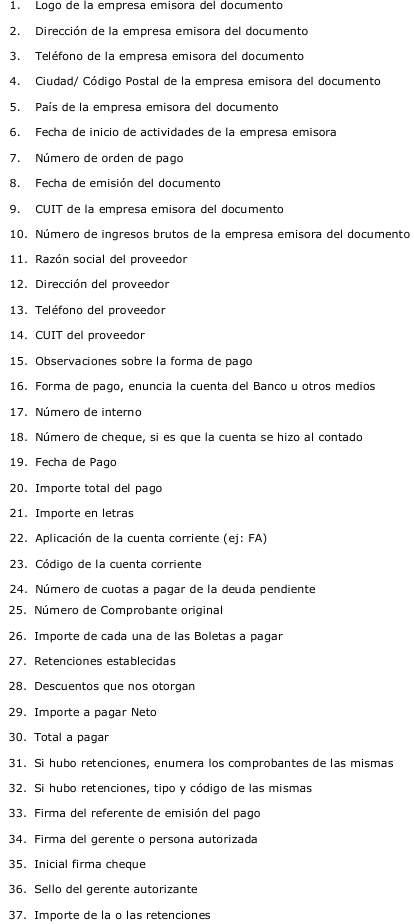
\includegraphics[keepaspectratio=true]{./Circuitos-Teoricos/Pago-a-Proveedores/Images/descripcion-orden-de-pago.png}
 % descripcion-pago-a-proveedores.png: 414x595 pixel, 96dpi, 10.95x15.74 cm, bb=0 0 310 446
\end{center}

\pagebreak
\subsection{Cheque}
\begin{center}
 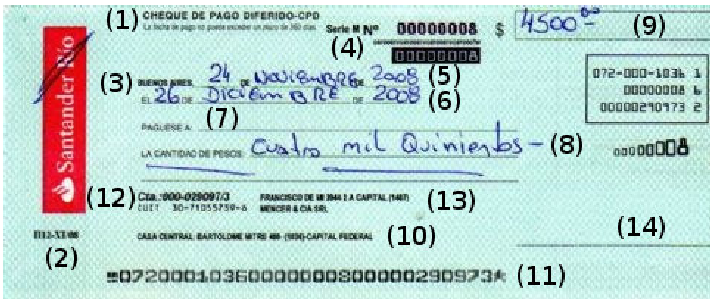
\includegraphics[scale=0.9,keepaspectratio=true]{./Circuitos-Teoricos/Pago-a-Proveedores/Images/cheque.png}
 % cheque.png: 713x304 pixel, 96dpi, 18.86x8.04 cm, bb=0 0 535 228
\end{center}

\begin{itemize}
  \item \textbf{Objetivo:} Con este documento se efectúa el pago. Se entrega al proveedor, y éste por intermedio de un depósito bancario o por ventanilla, obtiene el efectivo que el cheque representa.
  \item \textbf{Alcance:} Es un documento externo a la empresa.
  \item \textbf{Emisor:} Tesorería.
  \item \textbf{Cantidad de Copias Emitidas:} Original.
  \item \textbf{Sector receptor:} Gerencia Administrativa.
\end{itemize}

\textbf{Tipos de cheques}
\begin{itemize}
 \item \textbf{Cheque com\'un}
 \item \textbf{Cheque de pago diferido:} (Art\'iculo 52de la Ley 24.452) El cheque de pago diferido es una orden de pago librada a días vista, a contar desde su presentación para registro en una entidad autorizada, contra la misma u otra en la cual el librador a la fecha de vencimiento debe tener fondos suficientes depositados a su orden en cuenta corriente o autorización para girar en descubierto, dentro de los límites de registro que autorice el girado. La diferencia entre la fecha de emisión y la fecha de vencimiento no puede superar os 365 días.Sin perjuicio de las responsabilidades en que incurra por el derecho común, bajo ninguna circunstancia el girado será responsable si el cheque no es pagado a su vencimiento. Ni el registro del cheque, ni la determinación de límites de registro generan responsabilidad.El girado puede avalar el cheque de pago diferido.
 \item \textbf{Cheque cruzado:} (Art\'iculo 44 de la Ley 24.452) El librador o el portador de un cheque pueden cruzarlo con los efectos indicados en el artículo siguiente. El cruzamiento se efectúa por medio de dos barras paralelas colocadas en el anverso del cheque. Puede ser general o especial. El cruzamiento es especial si entre las barras contiene el nombre de una entidad autorizada para prestar el servicio de cheque, de lo contrario el cruzamiento es general. El cruzamiento general se puede transformar en cruzamiento especial; pero el cruzamiento especial no se puede transformar en cruzamiento general. La tacha del cruzamiento o de la mención contenida entre las barras se tendrá por no hecha. En consecuencia el cheque cruzado solo se cobra a través de un banco, depositándolo.
\end{itemize}

\subsubsection{Descripción}
\begin{center}
 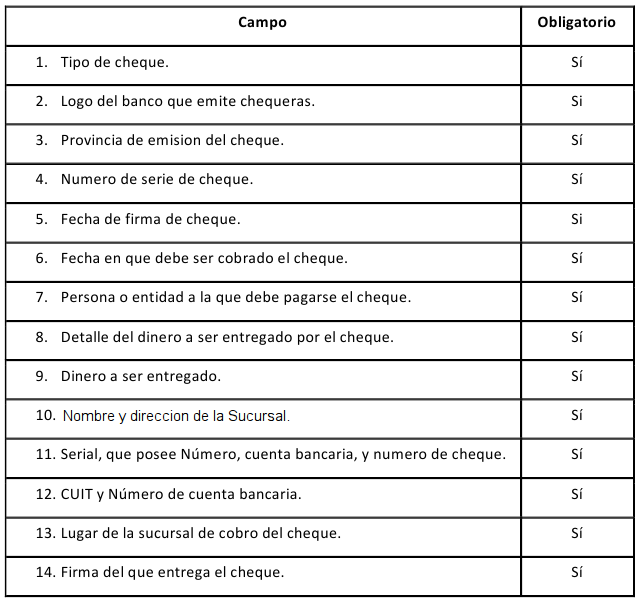
\includegraphics[scale=0.9,keepaspectratio=true]{./Circuitos-Teoricos/Pago-a-Proveedores/Images/descripcion-cheque.png}
 % descripcion-cheque.png: 640x366 pixel, 96dpi, 16.93x9.68 cm, bb=0 0 480 274
\end{center}

\pagebreak
\section{Normas de control interno generales y específicas de Pagos a Proveedores}
\begin{enumerate}
  \item \textbf{Separación de funciones:}
El manejo de los fondos no debe estar a cargo de la misma persona que realiza la registración.  No es conveniente que el cajero realice la registración contable de donde surge el saldo por el cual es responsable, aunque es posible que para su control y para confeccionar las rendiciones que eleva al área contable tenga que efectuar algunas anotaciones.   En el caso particular de los Pagos, la liquidación y autorización debe ser realizada por una persona responsable ajena a Tesorería.
  \item \textbf{Concentración de la responsabilidad:}
Una sola persona será responsable de la custodia y del manejo de fondos, esa persona suele ser el Tesorero.
  \item \textbf{Separación total de los fondos:}
Para un control eficaz de los fondos es recomendable que los provenientes de cobranzas estén separados de los destinados a pagos,  por lo tanto, los valores que tienen origen en las cobranzas se depositaran en su total en la cuenta corriente bancaria y los pagos se efectuaran mediante cheques emitidos contra esa cuenta bancaria.
  \item \textbf{Rotación del personal:}
De manera que se puedan detectar posibles errores en el sistema.  Además, es aconsejable que este personal tome sus vacaciones anuales y que otra persona de la organización esté capacitada para realizar su reemplazo, como así también en casos de enfermedad o egreso del personal.  Los reemplazos se realizaran con personal ajeno al sector y que no tenga amistad o subordinación directa con el reemplazado.
  \item \textbf{Contabilización de las operaciones:}
De manera que permitan el control de las mismas y la consistencia con la información de otros sectores, por ejemplo, total de débitos o créditos en cuentas de terceros.  La registración estará respaldada por la documentación correspondiente.
  \item \textbf{Arqueos sorpresivos:}
Se realizan para verificar si los valores en existencia coinciden con los que surgen de la registración contable.
  \item \textbf{Conciliación bancaria}
\end{enumerate}

\subsection{Normas Específicas}
\begin{itemize}
  \item \textbf{Uso del Cheque:}
  \begin{itemize}
    \item Permite disminuir el riesgo que implica la tenencia de dinero en efectivo.
    \item Ejerce un mejor control sobre los pagos debido a que se podrán conciliar con el resumen bancario.
    \item Deben tomarse en cuenta las distintas modalidades que permite la legislación vigente: Ley 24.452 (Ley de Cheques).
    \item Los cheques deben ser firmados por dos responsables de la organización.
    \item Los cheques que se anulen deben quedar adheridos a la libreta de cheques o destruirse el ángulo inferior derecho donde se firma o en la parte donde figura su numeración.
  \end{itemize}


Con esta forma se persiguen dos finalidades:
  \begin{itemize}
    \item Que exista un control reciproco entre los firmantes y de esta manera detectar errores antes de que el pago se haga efectivo. Esto implica que los dos responsables que firman el cheque efectúen una revisión de la documentación respaldatoria y la inicialicen, puesto que de lo contrario esta norma no tendrá sentido.
    \item Se evita que una sola persona pueda disponer del uso indiscriminado de los fondos, con el consecuente riesgo que ello implica.
  \end{itemize}

  \item \textbf{Pago amparado con la totalidad de los comprobantes y anulación de los mismos:}
En el momento de confeccionar el cheque, la persona responsable tendrá a la vista la
documentación respaldatoria que le da origen y se le colocará el sello de “Pagado” y el
número del cheque con el que se efectúo el pago con el objeto de que no vuelva a ser
presentada para justificar o respaldar otro pago. Quienes firmen el cheque deberán
controlar que se cumpla con estos aspectos.
  \item \textbf{Existencia de fondo fijo o caja chica:}
Tendrá un monto estipulado previamente para realizar los pagos menores en efectivo, estará
a cargo de una persona responsable y su reposición se efectuara periódicamente mediante
la emisión de un cheque previa presentación de los comprobantes que respalden los pagos
efectuados.
  \item \textbf{Pagos de sueldos y jornales:}
Es importante que exista una separación de tareas entre quien controla la asistencia, quien
prepara la liquidación de los haberes y quienes efectúa el pago. En este caso, es de
especial interés la seguridad del movimiento de fondos para el pago (seguros de dinero en
transito, traslado por empresas especializadas, etc.). El pago al empleado se realiza previa
identificación y contra la entrega del recibo firmado.
\end{itemize}
